%% chapter-1: 绪论部分
%% 介绍本研究课题的学术背景及理论与实际意义,国内外文献综述,
%% 本研究课题的来源及主要研究内容。

\chapter{注释、图表、公式和计量单位格式}
论文中常常要用注释、图表、公式和计量单位表达研究工作内容。除了要注重论文结构的规范性,规范的注释、图表、公式和计量单位格式同样是论文质量的基本保证。
\section{注释}
注释是正文中为了不中断或割离连贯的叙述语言而对文中某些内容(如词语、内涵、引文出处、资料来源等)加以必要说明的文字。在论文写作中常用到的注释有注释表、脚注、图注和表注。注释表是指论文中符号、标志、缩略词、首字母缩写、计量单位、名词、术语等的注释汇集说明。这些文字按页排在页下方的叫脚注;排在图题下方或表格下方的叫图注或表注,这些都放在正文中[2]。

脚注用6号字排在相应正文同一页最下部。脚注按在同一页中出现的先后,在被注文字右上角依次编排序号,如\textcircled{1}、\textcircled{2}…。序号标示位置应紧靠被注文字,若被注文字后紧跟有标点符号,当此标点是顿号和逗号时,注序号放在标点符号前;其他标点符号,应根据被注释内容确定放在标点符号之前或之后。注文的序号应与文中所注序号相同。注文与正文之间用脚注线(细线,顶格排,长约版心宽度的四分之一)隔开。各条注文单列,均缩进两格起排,转行顶格,句末加句号。同一页正文中出现相同内容的注释时,第二次及其以后序号应与第一次相同,不必再顺序编号和重复加注文[2]。脚注的示例见1.3节。图注和表注的具体用法在3.2节中介绍。



\section{图表格式}
\subsection{图格式}
图包括曲线图、构造图、示意图、图解、框图、流程图、记录图、布置图、地图照片、图版等。学位论文的插图、照片必须确保能复制或微缩,以矢量图为最佳,且原则上应使用矢量图(尤其是来源本来就是图形工具绘制的矢量图)。

图应有“自明性”,即只看图、图题和图注,不阅读正文,就可以理解图意。如图3.1所示,图应编排序号。图的编号一律用阿拉伯数字依序连续编排,序号分章依序编号,其标注形式应便于互相区别,例如:图1.1、图1.2、图3.1、图3.2等。每一章图的编号应连续。如某章只有一幅图时,仍应标为“图×.1”。

图要有图题,是简短确切的题名,中文字体为宋体5号字,并置于图的编号之后,图的编号和图题应置于图下方的居中位置。\\


\begin{figure} 
	\centering
	\begin{minipage}[t]{0.8\linewidth} 
		\centering 
		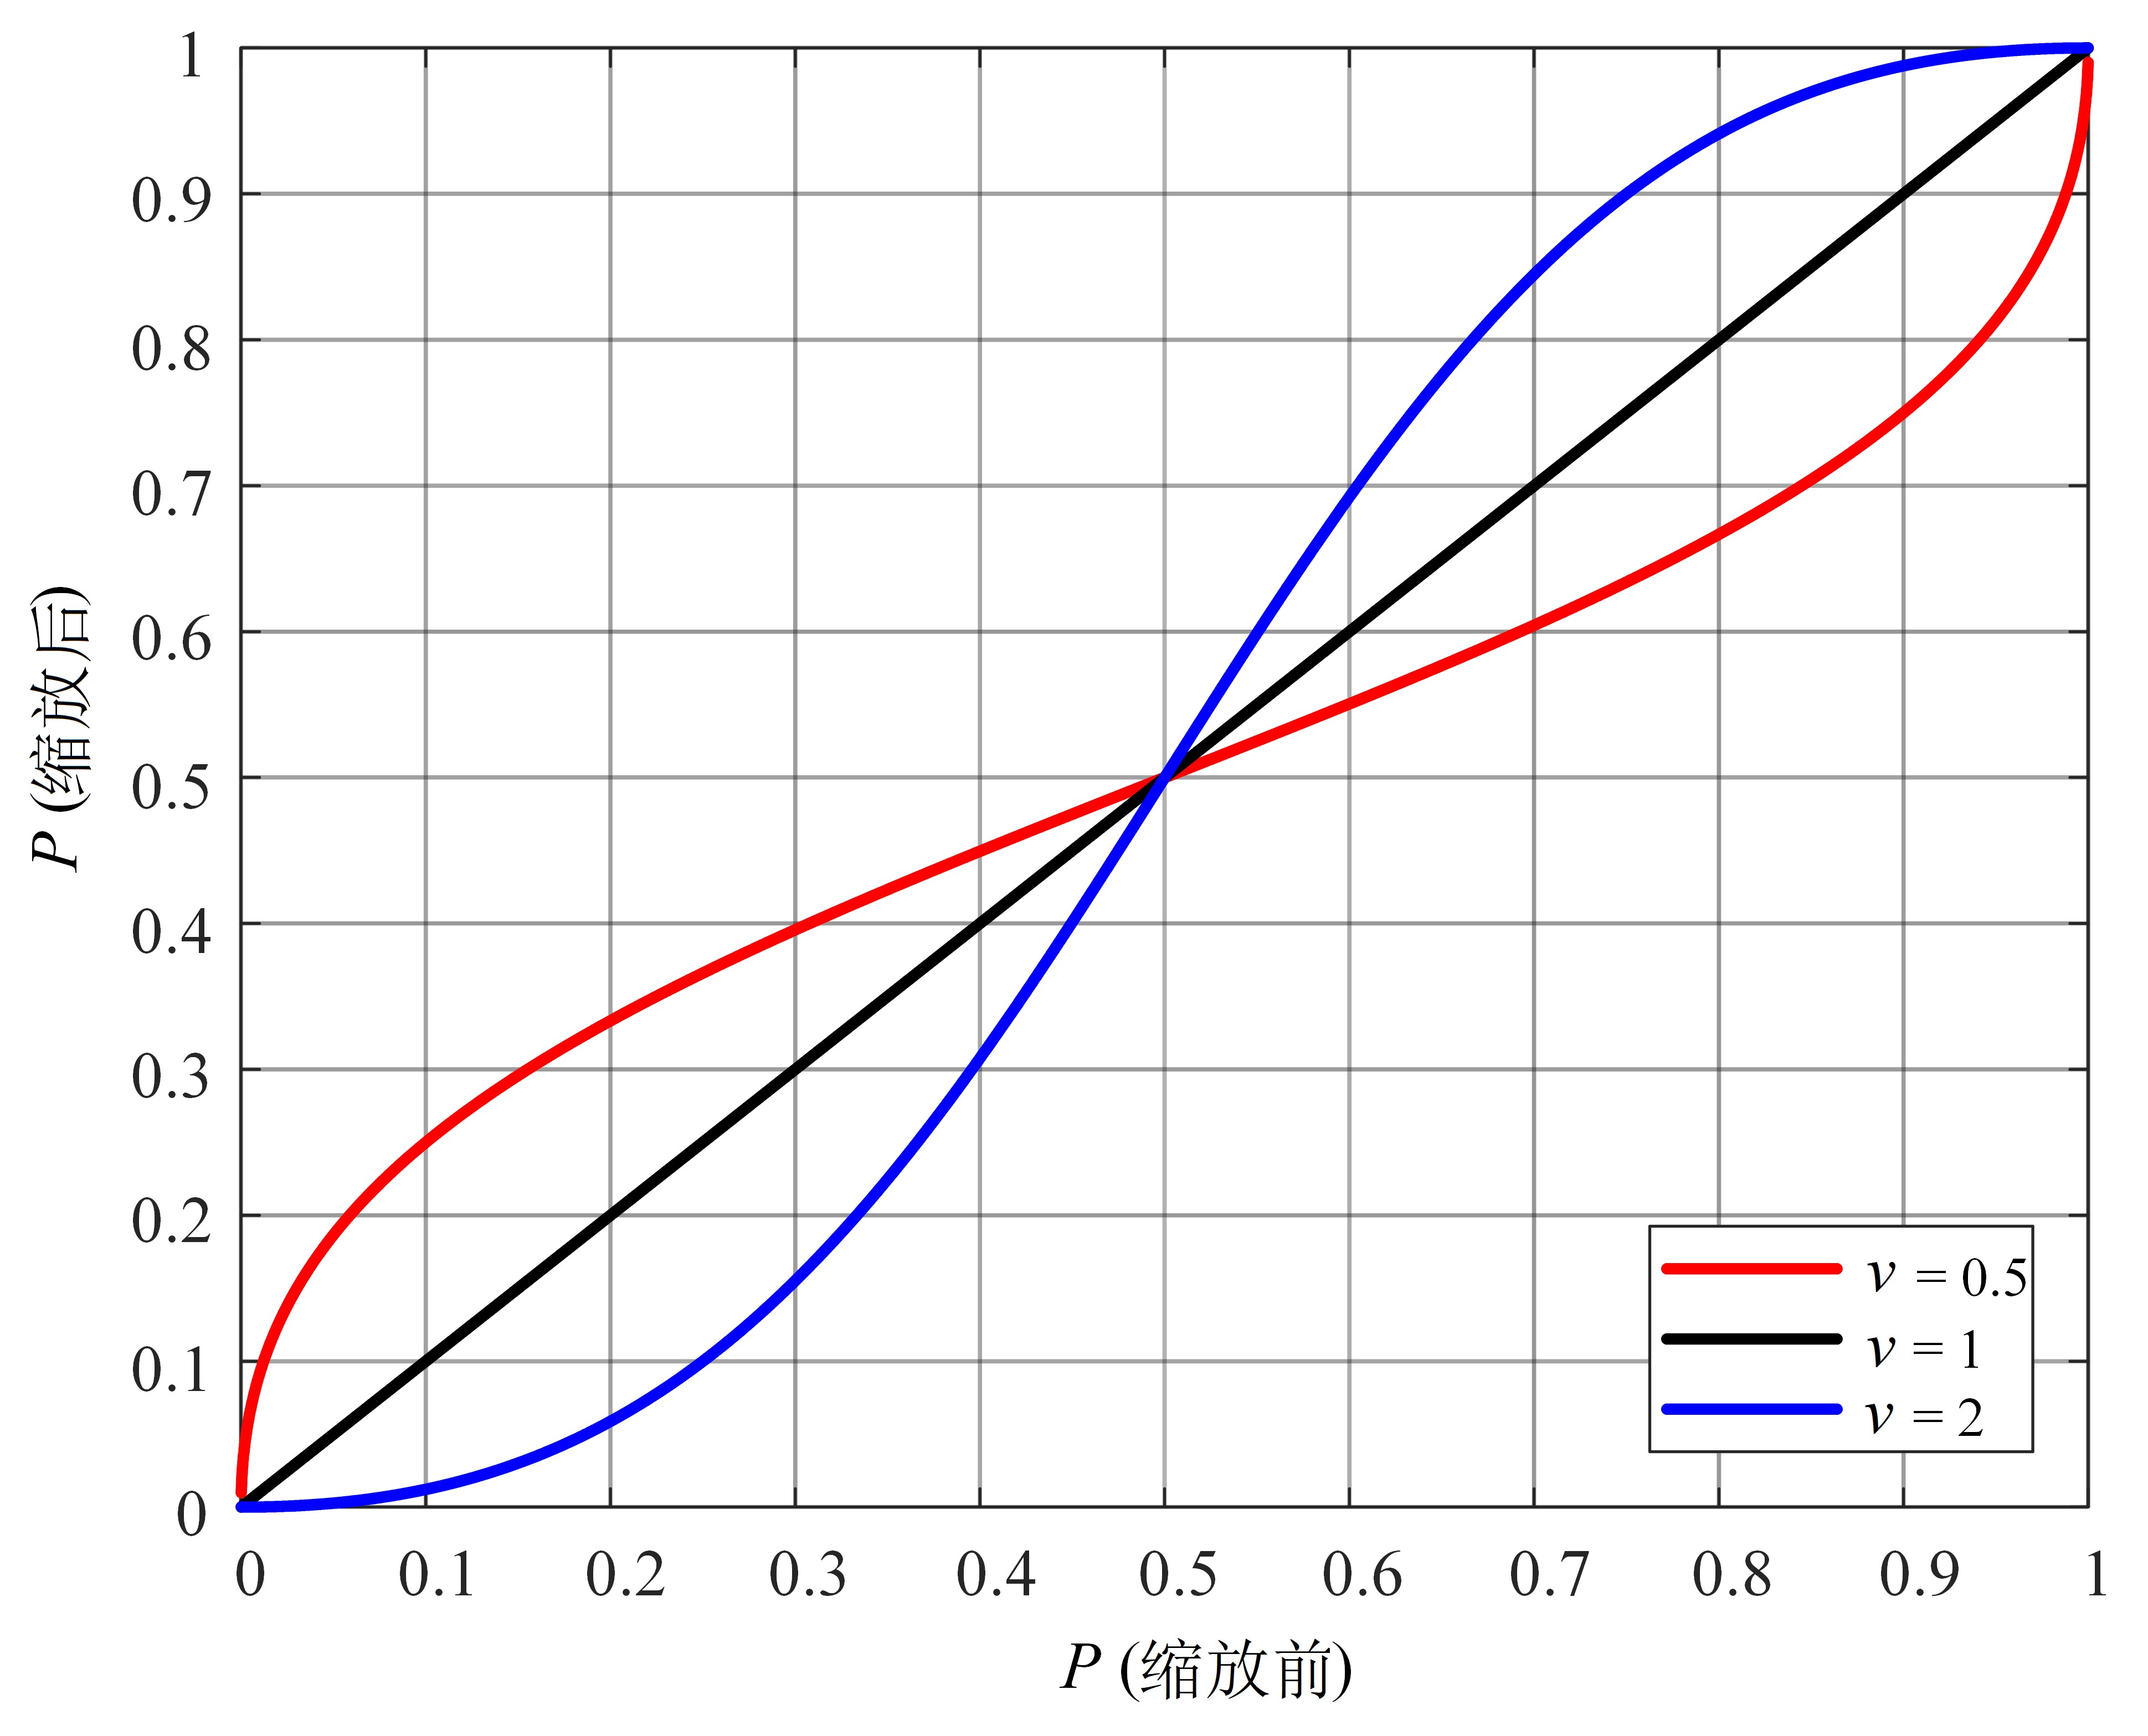
\includegraphics[width=10cm]{chapters/31}
		\caption{不同躲避角度下的Swarm-MAD模型群体与障碍中心平均距离\upcite{王兰芬2010Swarm}} 
		\label{fig:3.1} 
	\end{minipage}% 
\end{figure}

必要时,图还要有图注。图注指对图中的符号、标记、代码,以及实验条件等项目作补充说明或解释的简明文字。当插图的图元过多而不方便用文字注释时,在图中改用图元代号(往往用外文字母的大小写或正斜体、数字来表示不同系列的代号);在图外,即图题下放置图元代号的说明(即图注)。图注通常排在图题下方。图注的字号为6号。注释或说明图中项目时,其符号、阿拉伯数字、外文字符等,必须与图中一一对应。并列注释时,各项目通常用分号分开;句子较长,或一项注释中已有分号或句号时,各项间只能用句号分开,不能再用分号。图注应编排序号,注的序号以同一页内出现的先后次序单独排序,用\textcircled{1}、\textcircled{2}、\textcircled{3}…依次标示在需加注处[2]。

图与图题与正文之间空一行。分图题置于分图之下,分图号用(a)、(b)等表示,图3.2和图3.3为包含分图的图设置规范。图应居中,容易出现问题是图所在行出

图与图题与正文之间空一行。分图题置于分图之下,分图号用(a)、(b)等表示,图3.2和图3.3为包含分图的图设置规范。图应居中,容易出现问题是图所在行出现缩进,而导致图没有真正居中。多图要均匀排列,可利用虚框表格控制格式,如图3.2。



\begin{figure} 
	\centering 
	\subfigure[平均个体聚类度变化图]{ 
		\label{fig:subfig:a} %% label for first subfigure 
		\includegraphics[width=5.5cm]{chapters/32a}} 
	\hspace{1in} 
	\subfigure[邻域个体分布指数变化图]{ 
		\label{fig:subfig:b} %% label for second subfigure 
		\includegraphics[width=5.5cm]{chapters/32b}} 
	\caption{标示群体突现时刻的指标变化图[5]} 
	\label{fig:subfig} %% label for entire figure 
\end{figure}

\begin{figure} 
	\centering 
	\subfigure[θ = 0°(原模型)]{ 
		\label{fig:subfig:a} %% label for first subfigure 
		\includegraphics[width=10cm]{chapters/33a}} 
	\hspace{1in} 
	\subfigure[θ= 5°,25°,45°]{ 
		\label{fig:subfig:b} %% label for second subfigure 
		\includegraphics[width=10cm]{chapters/33b}} 
	\caption{带突现控制的Swarm-MAD群体代数连通度变化图[5]} 
	\label{fig:subfig} %% label for entire figure 
\end{figure}

曲线图的纵横坐标必须标注“量、标准规定符号、单位”。此三者只有在不必要标明(如无量纲等)的情况下方可省略。坐标上标注的量的符号和缩略词必须与正文一致。

照片图要求主题和主要显示部分的轮廓鲜明,便于制版。如用放大缩小的复制品,必须清晰反差适中。照片应有表示物尺寸的标度。

引用图应在图注中标出文献资料来源。

文中必须有关于本插图的提示,如“见图1.1”、“如图1.1所示”等。该页空白不够排写该图整体时,则可将其后文字部分提前排写,将图移到次页。

可以根据图的大小,将两个图并列放置,如图3.4和图3.5所示。


\begin{figure} 
	\begin{minipage}[t]{0.45\linewidth} 
		\centering 
		\includegraphics[width=7cm]{chapters/34} 
		\caption{个体与障碍中心平均距离[5]} 
		\label{fig:side:a} 
	\end{minipage}% 
	\begin{minipage}[t]{0.6\linewidth} 
		\centering 
		\includegraphics[width=7cm]{chapters/35} 
		\caption{个体到障碍影响范围边界平均距离[5]} 
		\label{fig:side:b} 
	\end{minipage} 
\end{figure}


\subsection{表格式}
表的编排一般是内容和测试项目由左至右横读,数据依序竖读。表应有自明性。表应编排序号,编号方式与图编号方式相同。例如:表1.1、表1.2、表3.1、表3.2等。

表要有表题,是简短确切的题名,并置于表的编号之后,表的编号和表题应置于表上方居中位置。必要时,应将表上的符号、标记、代码,以及需要说明事项等,用最简练的文字,横排于表题下,作为表注。表注应编排序号,与图注相同。

表注主要包括三种情况:资料来源(说明表中数据的文献来源,可用标题上引用参考文献、表下说明出处或脚注三种方式之一给出)、普通注解(对表中的数据处理的说明)、特殊注解(对某一个或几个表栏项目进行特别说明),如表3.1所示。表注通常用与表格内容相同的字体字号排在表格下方。表注的标号既可以表题与表内连续编号,用\textcircled{1} \textcircled{2}…标注在被注文字的右上角,也可以表题用“注:”或“*”号,表内用\textcircled{1} \textcircled{2}…分别编序号。无论采用哪种形式,全文要统一[2]。其中,采用参考文献引用方式时,该参考文献应符合参考文献要求(具体见第6章规定)。如仅引用少量内容,和本文工作相关度不大,应采用另外两种方式给出出处。

\begin{table}[h]
	\centering
	\caption[表3.1]{电流类型对效率的影响}
	\label{biao3.1}
	\begin{tabular}{m{4cm} m{3cm} m{3cm} m{3cm}}
		\hline 
		\makecell[c]{\textbf{电流类型}} & & & \makecell[c]{\textbf{$\frac{{{n_g}}}{\% }$}}\\ 
		\hline 
    	\makecell[c]{${J^2}(t) = 1$}	&\makecell[c]{4.27}  & \makecell[c]{1.28} & \makecell[c]{43.9(30)}\\ 
		\makecell[c]{${J^2}(t) = 1$}	&\makecell[c]{4.64}  & \makecell[c]{1.39} & \makecell[c]{41.8(29)}\\ 
    	\makecell[c]{${J^2}(t) = \frac{1}{t}$}	&\makecell[c]{3.28}  & \makecell[c]{0.98} & \makecell[c]{50.5}\\
		\hline 
	\end{tabular} 
\end{table}
资料来源:Wang Ying et al.2004.Physics of Electric Launch.Science Press。

文中必须有关于表的提示,可用“见表1.1”、“如表1.1所示”等。如“两种模型应用下球队与UVA球队的比赛结果如表3.2所示。”

%合并行:\multicolumn{n}{c}{ABCD...},其中n是要合并的格数
%合并列:\multirow{n}{*}{ABCD...},其中n是要合并的格数

%合并行和列:\multicolumn{n}{c}{\multirow{n}{*}{ABCD...}}   \\ \hline
%插入横线\cmidrule(lr){1-4} \cmidrule(lr){5-8} \\ \cline{2-4} 
% Please add the following required packages to your document preamble:
% \usepackage{multirow}
\begin{table}[]
	\caption[表3.2]{球队的比赛结果统计表[5]}
	\label{biao3.2}
	\begin{tabular}{cccccc}
		\hline
		\multirow{2}{*}{模型}       & \multirow{2}{*}{d} & \multirow{2}{*}{r} & \multirow{2}{*}{与对方队员的警戒距离} & \multicolumn{2}{c}{改进球队 VS UVA球队} \\ \cline{5-6} 
		&                    &                    &                             & 比分           & 拿球进攻时间             \\ \hline
		\multirow{4}{*}{Swarm}    & 10.0               & 5.0                &                             & 0:6          & 3978:2014          \\ 
		& 30.0               & 10.0               &                             & 0:4          & 2754:3010          \\ 
		& 50.0               & 10.0               &                             & 0:5          & 3174:2806          \\  
		& 70.0               & 10.0               &                             & 0:0          & 3113:2856          \\\hline
		\multirow{3}{*}{Swarm-OA} & 70.0               & 10.0               & 10.0                        & 1:2          & 3132:2794          \\
		& 70.0               & 10.0               & 70.0                        & 0:3          & 3180:2772          \\
		& 70.0               & 10.0               & 50.0                        & 0:1          & 2858:3012         \\ \hline
	\end{tabular} 
\end{table}

表名中不允许使用标点符号,表名后不加标点。表名与正文之间空一行。数字空缺的格内加横线“-”(占2个数字宽度)。

表内文字或数字上、下或左、右相同时,采用通栏处理方式(合并单元格),表内文字或数字上、下或左、右相同时,采用通栏处理方式(合并单元格),或一律填上具体数字或文字,不允许用“〃”、“同上”之类的写法。

表内文字说明,起行空一格、转行顶格、句末不加标点。

表的各栏应标明“量、标准规定符号、单位”。此三者只有在不必要标明(如无量纲等)情况下方可省略。表中的缩略词和符号,必须与正文一致。

如某个表需要转页接排,在随后的各页上应重复表的编号。编号后跟表题(可省略)和“(续)”,如“表1.1 xxxx(续)”或“表1.1(续)”所示,续表均应重复表头和关于单位的陈述。编号后加“(续表)”,表题可省略。续表应重复表头[2]。
 
表格不加左、右边线。表的编排建议采用国际通行的三线表或不完全表。其中,三线表通常只有3条线,即顶线、底线和栏目线,没有竖线,以其形式简洁、功能分明、阅读方便而在科技论文中被推荐使用,如表3.1和3.2。不完全表是指有其余表线,没有左右两根边线的表格,如表2.1和表2.2(为区别表内容和表头,此时表头文字可加粗)。可根据内容采用两种形式之一,以形式简洁但不带来阅读者理解困难为前提。附录A使用了常见的完全表(即所有表线不省略)。

表题、表内文字和表注一般均为宋体5号字,单倍行距。根据内容多少,为保证一行排版,也可适当减小字号或紧缩字体排版。表中单元格的间距合适,紧促美观。

\section{公式格式}
正文中的公式、算式或方程式等应注明编号,按章顺序编排,公式的编号右端对齐(当有续行时,应标注于最后一行),公式与编号之间用空格连接。公式中字符大小合适,基本字符大小与正文匹配,为小4号。即一个变量在正文中是小4号,那么公式中显示效果与之一致,也应为小4号字体,上、下标等字符等参照此字号减小。

公式应另起一行居中排,公式较长时最好在等号“=”处转行,如难实现,则可在+,-,×,÷,<,>等运算符号处转行,转行时运算符号仅书写于转行式前,不重复书写。上下式在符号“=”处对齐。

公式中第一次出现的物理量代号应给予注释,注释的转行应与破折号“——”后第一个字对齐。破折号占二个字,注释物理量需用公式表示时,公式后不应出现公式序号。公式下面的“式中”空两个字起排,单独占一行。公式中所要解释的符号按先左后右,先上后下顺序分行空两个字排,再用破折号与释文连接,回行时与上一行释文对齐。上下行的破折号对齐。

公式中应注意分数线的长短(主、副分数线严格区分),长分数线与等号对齐。


示例1:
\begin{equation}
    a = {a_{\max }}\frac{v}{{\left| v \right|}}  \label{gongshi3.1}  %\ref{gongshi3.1}引用公式
\end{equation}

其中:(注:留意此段不应缩进,和上行属于同一段。这是论文常见问题。)

\begin{equation}
v = {c_1}{v_1}(d) + {c_2}{v_2}(d) + {c_3}{v_3}(d) + {c_4}{v_4}(d) + {c_5}{v_5}(d) \label{gongshi3.2}
\end{equation}

式中,$ c_{1}~c_{5}$——各项的权值,常数

     \hspace*{1.1cm}  ${v_r}$——单位随机向量
     
     示例2:
     
     {\large $x = \frac{{2\pi ({n_1} + {n_3})}}{{\frac{{{n_1} + {n_2}}}{{{n_1} - {n_2}}}}}$}
     
     
\section{计量单位格式}

文中所用的物理量和单位一律采用《中华人民共和国法定计量单位》,并遵照《中华人民共和国法定计量单位使用方法》(GB3100~3102-93)。单位名称和符号的书写方式一律采用国际通用符号,全文统一。物理量用斜体,单位用正体。

\section{本章小结}

介绍了论文中出现的注释、图表、公式和计量单位的格式,以及在图表中注释,即图注和表注的标注方法,供撰写论文时参照执行。 
